\section{Vectors and Linear Combination}
\label{sec:vectors_and_linear_combination}

\paragraph{Linear Combination}
Vectors $v$ and $w$ are both 2D vectors. The linear combination of $v$ and $w$ are
the vectors $cv + dw$ for any scalars $c$ and $d$.:
\[
	v =
	\begin{bmatrix}
		v_{1} \\
		v_{2}
	\end{bmatrix}
	=
	\begin{bmatrix}
		2 \\
		4
	\end{bmatrix}, \quad w = \begin{bmatrix}w_{1} \\ w_{2} \end{bmatrix}=
	\begin{bmatrix}
		1 \\
		3
	\end{bmatrix}
\]

\noindent
The linear combinations $c
	\begin{bmatrix}
		2 \\
		4
	\end{bmatrix}
	+ d
	\begin{bmatrix}
		1 \\
		3
	\end{bmatrix}
	=
	\begin{bmatrix}
		2c + 1d \\
		4c + 3d
	\end{bmatrix}$ form $xy$ plane. \\

\noindent
$v$ and $w$ are \textbf{linearly independent}. There is exactly one solution
$b_{1}$, $b_{2}$. \\

\noindent
The 2 by 2 matrix $A =
	\begin{bmatrix}
		v & w
	\end{bmatrix}$ is \textbf{invertible}.

\begin{mdframed}
	\textbf{Column Way, Row Way, Matrix Way} \\
	\noindent
	Column way, Linear combination:
	\[
		c
		\begin{bmatrix}
			v_{1} \\
			v_{2}
		\end{bmatrix}
		+ d
		\begin{bmatrix}
			w_{1} \\
			w_{2}
		\end{bmatrix}
		=
		\begin{bmatrix}
			b_{1} \\
			b_{2}
		\end{bmatrix}
	\]

	\noindent
	Row way, Two equations for $c$ and $d$:
	\[
		v_{1}c + w_{1}d = b_{1}, \quad v_{2}c + w_{2}d = b_{2}
	\]

	\noindent
	Matrix way, 2 by 2 matrix:
	\[
		\begin{bmatrix}
			v_{1} & w_{1} \\
			v_{2} & w_{2}
		\end{bmatrix}
		\begin{bmatrix}
			c \\
			d
		\end{bmatrix}
		=
		\begin{bmatrix}
			b_{1} \\
			b_{2}
		\end{bmatrix}
	\]
\end{mdframed}

\paragraph{Vectors in 3D}
We need \textit{three} independent vectors to span 3D space $R^3$.

\begin{mdframed}
	\textbf{Identity Matrix $I$:} denoted by $I_n$ for an $nxn$ identity matrix, where $n$ is the number of rows or columns.
	\[
		I_3 =
		\begin{bmatrix}
			1 & 0 & 0 \\
			0 & 1 & 0 \\
			0 & 0 & 1
		\end{bmatrix}
	\]
	Multiplying any matrix by $I$ leaves the matrix unchanged. $I$ is the matrix
\end{mdframed}
\label{sec:vectors_and_linear_combination_end}

\section{Length and Angles from Dot Products}
\paragraph{Dot Product} The dot product of two vectors $v=\begin{bmatrix}
		v_{1} \\
		v_{2}
	\end{bmatrix}$ and $w=\begin{bmatrix}
		w_{1} \\
		w_{2}
	\end{bmatrix}$ is $v \cdot w = v_{1}w_{1} + v_{2}w_{2} = w \cdot v$ .

\paragraph{Unit Vector} A unit vector is a vector with length 1. The unit vector in the direction of $v$ is $\dfrac{v}{\|v\|}$.

\paragraph{Perpendicular Vectors} Two vectors $v$ and $w$ are perpendicular if $v \cdot w = 0$.
\[
	\|v + w\|^2 = (v + w) \cdot (v + w) = v \cdot v + 2v \cdot w + w \cdot w = \|v\|^2 + \|w\|^2
\]
\[
	\|v - w\|^2 = (v - w) \cdot (v - w) = v \cdot v - 2v \cdot w + w \cdot w = \|v\|^2 + \|w\|^2
\]

\paragraph{Angle between Vectors} The angle between two vectors $v$ and $w$ is $\theta = \cos^{-1} \left( \dfrac{v \cdot w}{\|v\| \|w\|} \right)$.

\begin{example}\textnormal{
		The unit vectors $v=(\cos \alpha, \sin \alpha)$ and $w=(\cos \beta, \sin \beta)$ have $v \cdot w = \cos \alpha \cos \beta + \sin \alpha \sin \beta$. In trigonometry, this is the formula for $\cos (\alpha - \beta)$ or $\cos (\beta - \alpha)$.}

	\begin{figure}[h!]
		\centering
		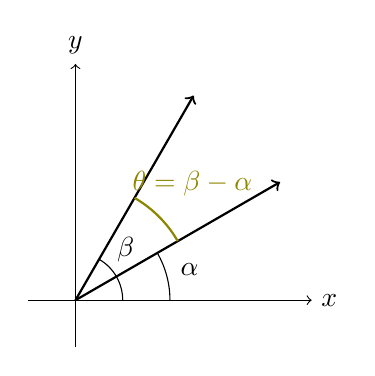
\begin{tikzpicture}[scale=3]
			% Draw axes
			\draw[->] (-0.2, 0) -- (1, 0) node[right] {$x$};
			\draw[->] (0, -0.2) -- (0, 1) node[above] {$y$};

			% Draw angle beta
			\draw[->, thick, black] (0,0) -- (30:1cm);
			\draw[->, thick, black] (0,0) -- (60:1cm);

			% % Mark angles (cosine)
			% Mark arc for be (smaller radius)
			\draw (0.4cm, 0) arc (0:30:0.4cm);  % arc for be (lower)
			\node at (15:0.5cm) {$\alpha$};

			% Mark arc for beta (larger radius)
			\draw (0.2cm, 0) arc (0:60:0.2cm);  % arc for beta
			\node at (45:0.3cm) {$\beta$};

			% Mark arc for theta (same radius as beta)
			\draw[thick, olive] (30:0.5cm) arc (30:60:0.5cm);  % arc for theta
			\node[olive] at (45:0.7cm) {$\theta = \beta - \alpha $};

		\end{tikzpicture}
		\caption{Visualization of $\cos(\beta - \alpha) = \cos(\theta)$ in the unit circle.}
	\end{figure}

	\noindent\textnormal{For unit vectors, $\cos \theta = v \cdot w$.
		When $v$ and $w$ are not unit vectors, divide by their length to get $u = v/\|v\|$ and $U = u/\|u\|$ and turn them into unit vectors.}
\end{example}

\begin{mdframed}
	\textbf{Cosine Formula} \\
	If $v$ and $w$ are nonzero vectors then $\dfrac{v \cdot w}{\|v\|\|w\|} = \cos \theta$
\end{mdframed}

\noindent Since $|\cos \theta| \leq 1$, this cosine formula gives two great inequalities:
\begin{mdframed}
	\textbf{Cauchy-Schwarz Inequality} \\
	For any vectors $v$ and $w$, $|v \cdot w| \leq \|v\|\|w\|$.

	\vspace{0.1cm}
	\noindent\textbf{Triangle Inequality} \\
	For any vectors $v$ and $w$, $\|v + w\| \leq \|v\| + \|w\|$.
\end{mdframed}

\noindent The triangle inequality comes directly from the Schwarz inequality:
\[
	\|v + w \|^{2} = v^{2} + 2v \cdot w + w^{2} \leq v^2 + 2\|v\|\|w\| + w^2 = (\|v\| + \|w\|)^{2}
\] Take the square root of both sides to get $\|v + w\| \leq \|v\| + \|w\|$.

\section{Row and Column Spaces}


\paragraph{Column Space}
Think of the columns of $A$ as vectors $a_1$, $a_2$, ..., $a_n$. The column space of $A$ is the set of all possible combinations $Ax = x_1a_1 + x_2a_2 + \ldots + x_na_n$.

\paragraph{Row Space} The row space of $A$ is the set of all possible combinations of the rows of $A$. The row space is the same as the column space of $A^T$.

\section{Matrix Multiplication $AB$}

\[
	A = \begin{bmatrix}
		1 & 2 \\
		3 & 4
	\end{bmatrix} \quad
	B= \begin{bmatrix}
		5 & 6 \\
		7 & 8
	\end{bmatrix}
\]

\noindent We multiply $A$ with each column of $B$, $b_1$ and $b_2$, to produce columns of $AB$. We can multiply $Ab_1$ the \textit{row way} or the \textit{column way}. \\
\begin{mdframed}

	\noindent\textbf{Row way, Dot products}
	\[
		Ab_1 = \begin{bmatrix}
			1 & 2 \\
			3 & 4
		\end{bmatrix}
		\begin{bmatrix}
			5 \\
			7
		\end{bmatrix}
		=
		\begin{bmatrix}
			row 1 \cdot b_1 \\
			row 2 \cdot b_2
		\end{bmatrix}
		=
		\begin{bmatrix}
			1 \cdot 5 + 2 \cdot 7 \\ 3 \cdot 5 + 4 \cdot 7
		\end{bmatrix}
		=
		\begin{bmatrix}
			19 \\ 43
		\end{bmatrix}
	\]

	\noindent\textbf{Column way, Combine columns}
	\[
		Ab_1 = \begin{bmatrix}
			1 & 2 \\
			3 & 4
		\end{bmatrix}
		\begin{bmatrix}
			5 \\
			7
		\end{bmatrix}
		=
		5\begin{bmatrix}
			1 \\ 3
		\end{bmatrix}
		+ 7\begin{bmatrix}
			2 \\ 4
		\end{bmatrix}
		=
		\begin{bmatrix}
			5 \\ 15
		\end{bmatrix}
		+
		\begin{bmatrix}
			14 \\ 28
		\end{bmatrix}
		=
		\begin{bmatrix}
			19 \\ 43
		\end{bmatrix}
	\]
\end{mdframed}

\vspace{0.5cm}
\noindent\textbf{Four Ways to Multiply $AB = C$}

\noindent Suppose we have $A$ as a 3 by 2 matrix $A =
	\begin{bmatrix}
		1 & 2 \\
		3 & 4 \\
		5 & 6
	\end{bmatrix}$, $B$ as a 2 by 4 matrix $B = \begin{bmatrix}
		1 & 2 & 3 & 4 \\
		5 & 6 & 7 & 8
	\end{bmatrix}$, then $C$ is a 3 by 4 matrix. \\

\noindent\textbf{1. Dot product way} $\Rightarrow$ 12 numbers

\[(\text{Row} \; i \; \text{of} \; A) \cdot (\text{Column} \; j \; \text{of} \; B) = C_{ij}\]

\[
	AB =
	\begin{bmatrix}
		1 \cdot 1 + 2 \cdot 5 & 1 \cdot 2 + 2 \cdot 6 & 1 \cdot 3 + 2 \cdot 7 & 1 \cdot 4 + 2 \cdot 8 \\
		3 \cdot 1 + 4 \cdot 5 & 3 \cdot 2 + 4 \cdot 6 & 3 \cdot 3 + 4 \cdot 7 & 3 \cdot 4 + 4 \cdot 8 \\
		5 \cdot 1 + 6 \cdot 5 & 5 \cdot 2 + 6 \cdot 6 & 5 \cdot 3 + 6 \cdot 7 & 5 \cdot 4 + 6 \cdot 8
	\end{bmatrix}
	=
	\begin{bmatrix}
		11 & 14 & 17 & 20 \\
		23 & 30 & 37 & 44 \\
		35 & 46 & 57 & 68
	\end{bmatrix}
\]

\noindent\textbf{2. Column way} $\Rightarrow$ 4 columns

\noindent For column $j$ in $C$, we multiply $A$ by $B_{\text{col}_j}$:

\[C_{\text{col}_j} = A \cdot \text{Column} \; j \; \text{of} \; B\]

\noindent To calculate $C_{\text{col}_1}$:

\[
	C_{\text{col}1} = A \cdot \begin{bmatrix}
		1 \\ 5
	\end{bmatrix}
	=
	1 \cdot \begin{bmatrix}
		1 \\ 3 \\ 5
	\end{bmatrix}
	+ 5 \cdot \begin{bmatrix}
		2 \\ 4 \\ 6
	\end{bmatrix}
	=
	\begin{bmatrix}
		11 \\ 23 \\ 35
	\end{bmatrix}
\]

\noindent The same goes for columns 2, 3, and 4 of $C$.

\noindent\textbf{3. Row way} $\Rightarrow$ 3 rows

\noindent For row $i$ in $C$, we multiply $A_{\text{row}_i}$ by $B$:

\[
	C_{\text{row}_i} = \text{Row} \; i \; \text{of} \; A \cdot B
\]

\noindent To calculate $C_{\text{row}_1}$:

\[
	C_{\text{row}_1} = \begin{bmatrix}
		1 & 2
	\end{bmatrix} \cdot B
	=
	\begin{bmatrix}
		1 & 2
	\end{bmatrix} \cdot
	\begin{bmatrix}
		1 & 2 & 3 & 4 \\
		5 & 6 & 7 & 8
	\end{bmatrix}
	=
	\begin{bmatrix}
		11 & 14 & 17 & 20
	\end{bmatrix}
\]

\noindent The same goes for rows 2 and 3 of $C$.

\noindent\textbf{4. Matrix way} $\Rightarrow$ sum of 2 Rank 1 matrices

\begin{align*}
	C & = A_{\text{col}_1} \cdot B_{\text{row}_1} + A_{\text{col}_2} \cdot B_{\text{row}_2} \\
	  & = \begin{bmatrix}
		      1 \\ 3 \\ 5
	      \end{bmatrix} \cdot \begin{bmatrix}
		                          1 & 2 & 3 & 4
	                          \end{bmatrix}
	+ \begin{bmatrix}
		  2 \\ 4 \\ 6
	  \end{bmatrix} \cdot \begin{bmatrix}
		                      5 & 6 & 7 & 8
	                      \end{bmatrix}                                                    \\
	  & = \begin{bmatrix}
		      1 & 2  & 3  & 4  \\
		      3 & 6  & 9  & 12 \\
		      5 & 10 & 15 & 20
	      \end{bmatrix}
	+ \begin{bmatrix}
		  10 & 12 & 14 & 16 \\
		  20 & 24 & 28 & 32 \\
		  30 & 36 & 42 & 48
	  \end{bmatrix}                                                                     \\
	  & = \begin{bmatrix}
		      11 & 14 & 17 & 20 \\
		      23 & 30 & 37 & 44 \\
		      35 & 46 & 57 & 68
	      \end{bmatrix}
\end{align*}

\paragraph{Associative \& Distributive Law} Both associative and distributive laws apply to matrix multiplication.

\begin{mdframed}
	\textbf{Associative} \quad $(AB)C = A(BC)$ \\
	\textbf{Distributive} \quad $A(B + C) = AB + AC$
\end{mdframed}

\section{The Rank of a Matrix}

The rank of a matrix is the maximum number of linearly independent rows or linearly independent columns in that matrix.

\noindent \textbf{Rank-One Matrix:} A matrix where all rows (or columns) are linearly dependent on one another. Example:
\[
	A = \begin{bmatrix}
		1 & 2 \\
		2 & 4 \\
		3 & 6
	\end{bmatrix}
\]

\noindent\textbf{Rank-Two Matrix:} A matrix where there are two linearly independent rows (or columns). Example:
\[
	A = \begin{bmatrix}
		1 & 2 \\
		3 & 4 \\
		5 & 6
	\end{bmatrix}
\]
The two columns of $A$ are linearly independent. The three rows of $A$ are not all linearly independent, specifically, $r_3 = -r_1 + 2 r_2$. So the maximum number of linearly independent rows or columns is 2.

\begin{mdframed}
	\textbf{Row rank equals column rank for any matrix.}
\end{mdframed}


\section{$A = CR$}

$C$ represents a matrix of linearly independent columns of $A$. $R$ is a reduced matrix that expresses how the columns of $A$ can be reconstructed using the columns of $C$.

\paragraph{$C$ contains the First $r$ Independent Columns of $A$} Suppose we go from left to right, looking for independent columns of $A$:

\begin{itemize}
	\item If column 1 of $A$ is not all zero, put it into the matrix $C$
	\item If column 2 of $A$ is not a multiple of column 1, put it into $C$
	\item If column 3 of $A$ is not a combination of columns 1 and 2, put it into $C$. \textit{Continue}
\end{itemize}

\noindent$C$ will have $r$ columns, where $r$ is the rank of $A$ and $C$. The $r$ columns of $C$ are linearly independent.

\paragraph{Part of $R$ is the \textit{Identity Matrix}} This corresponds to the columns of $A$ that went straight into $C$. The remaining columns of $R$ contain the coefficients that express the dependent columns of $A$ as a combination of the columns of $C$.
\textbf{When a column of $A$ goes into $C$, a column of $I$ goes into $R$.}

\setcounter{example}{0}
\begin{example}
	\[
		A = \begin{bmatrix}
			a_1 & a_2 & 3a_1 + 4a_2
		\end{bmatrix}
		= \begin{bmatrix}
			a_1 & a_2
		\end{bmatrix}
		\begin{bmatrix}
			1 & 0 & 3 \\
			0 & 1 & 4
		\end{bmatrix}
		= CR
	\]
\end{example}

\paragraph{Find $R$ with Elimination} The elimination process is called \textit{row reduction}.
\[
	A = \begin{bmatrix}
		1 & 3 & 4 \\
		2 & 4 & 2 \\
		3 & 7 & 6
	\end{bmatrix}
	= \begin{bmatrix}
		1 & 3 \\
		2 & 4 \\
		3 & 7
	\end{bmatrix}
	\begin{bmatrix}
		1 & 0 & -5 \\
		0 & 1 & 3
	\end{bmatrix}
	= CR
\]

\noindent First perform $row_1 - row_2 \times 2$ and $row_3 - row_1 \times 3$ to get $B$.
Then perform $row_3 - row_2$ to get $U$.

\[
	A \rightarrow B = \begin{bmatrix}
		1 & 3  & 4  \\
		0 & -2 & -6 \\
		0 & -2 & -6
	\end{bmatrix}
	\rightarrow U = \begin{bmatrix}
		1 & 3  & 4  \\
		0 & -2 & -6 \\
		0 & 0  & 0
	\end{bmatrix}
	= \text{upper triangular matrix} \; U
\]

\noindent Eliminate upwards to produce more zeros in $U$. First divide row 2 by -2, then make the entry above the pivot element ($row_1, col_2$) equal to zero with $row_1 - 3 \times row_2$.
\[
	U = \begin{bmatrix}
		1 & 3  & 4  \\
		0 & -2 & -6 \\
		0 & 0  & 0
	\end{bmatrix}
	\rightarrow
	\begin{bmatrix}
		1 & 3 & 4 \\
		0 & 1 & 3 \\
		0 & 0 & 0
	\end{bmatrix}
	\rightarrow
	\begin{bmatrix}
		1 & 0 & -5 \\
		0 & 1 & 3  \\
		0 & 0 & 0
	\end{bmatrix}
	= R_0
\]
Removing the zero row of $R_0$ gives $R$.